\documentclass{article}
\usepackage{graphicx} % Required for inserting images
\usepackage{float}
\title{Lesson 15 Homework - Proof Writing}
\author{William Wang}
\date{December 2025}
\usepackage{amsmath}
\begin{document}

\maketitle

\section{}
Let \(A = (0,0), B = (14,0)\)First we want to find the vertex of the parabola defined by \(y = x^2-10x+37\). Since the x-coordinate of the vertex is defined by \(\frac{-b}{2a}\), we have the vertex of the parabola \(C = (5,12)\). Hence we know that the ellipse passes through \((5,12)\). Then we can calculate the distance from each of the foci to this point and we know that the sum of the distances is equal to the sum of the distances from the foci to any point.
\[AC = \sqrt{5^2+12^2} = 13\]
\[BC = \sqrt{9^2+12^2}=15\]
So then the sum of the distances is 28. Then we know that distance from the foci to the endpoints of one of the axes is also 14. Hence we have an equilateral triangle with the two foci and the endpoint of a axis. Let \(D \) be the centre of the ellipse. 
\[D = (7,0)\]
Then we can find the endpoints of that axis. 
\begin{figure}[H]
    \centering
    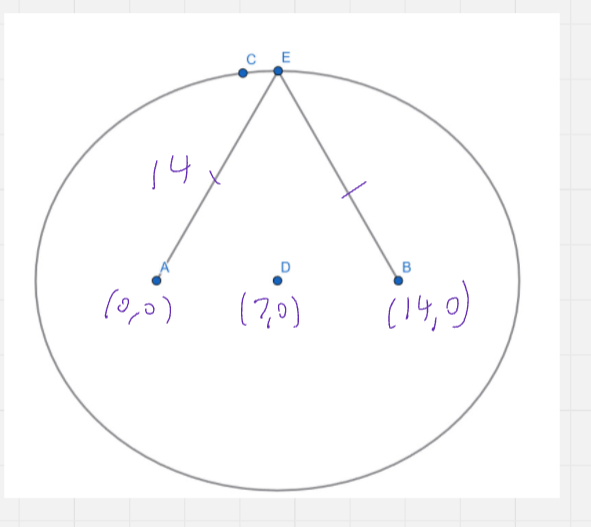
\includegraphics[width=0.5\linewidth]{q1a.png}
\end{figure}
\[ED = \sqrt{14^2 - 7^2} = \sqrt{147} \implies E = (7, \sqrt{147})\]
Then the other endpoint of the axis is \((7, -\sqrt{147})\). Hence one of the axes is 
\[EF = 2\sqrt{147}\]
\begin{figure}[H]
    \centering
    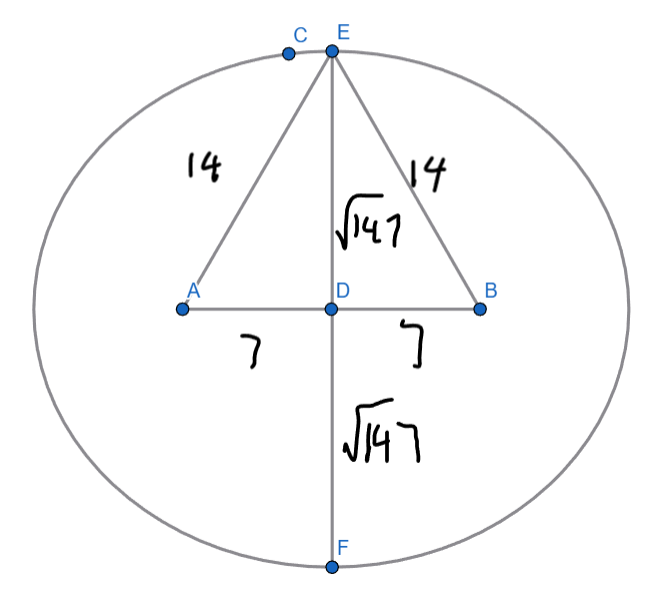
\includegraphics[width=0.5\linewidth]{q1b.png}
\end{figure}
For the other coordinate, we know it has to be in line with the two foci. Hence if we let one of the endpoints be $G$ then we know that
\[AG + BG=  28 \implies AB + 2AG = 28\]
\[AB = 14 \implies AG  = 7\]
\begin{figure}[H]
    \centering
    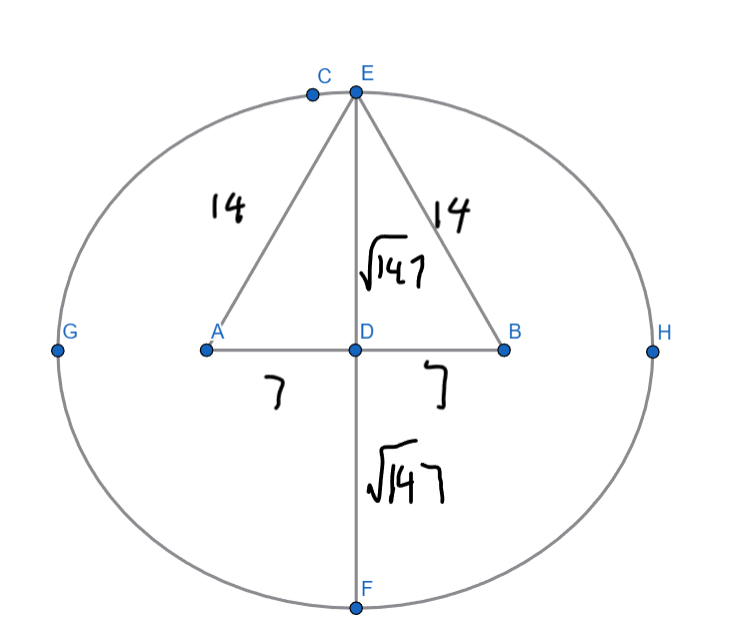
\includegraphics[width=0.5\linewidth]{q1c.png}
\end{figure}
Hence we have 
\[G = (-7,0) \text{ and } H = (21,0)\]
Then since the major axis is the longer one of those two. 
\[GH = 28 \text{ and } 12 \le EF \le 13\]
Hence $GH$ is the major axis and has a length of $28$. 


\section{}
Let $A = (6,5)$. We know that A must be the endpoint of the minor axis since it is horizontally in line with the foci. Let $F_1 = (4,1)$ and $F_2$ be the second foci, then we can find $F_2$ with the distance formula since we know that 
\[F_1 A = F_2 A\]
\[F_1 A = \sqrt{(6-4)^2 + (5-1)^2} = \sqrt{20} = 2\sqrt{5}\]
Then we have $F_2 = (x, 1)$ and since we know that \(F_2 A = 2\sqrt{5}\), we can solve for $x$. 
\[\sqrt{(6-x)^2 + (5-1)^2} = \sqrt{20} \implies x = 8\]
Hence we have the foci of the ellipse. 
\[F_1 = (4,1) \text{ and } F_2 = (8,1)\]
\[\text{Distance between foci } = 4\]
\[\text{Center of the ellipse } = (6,1)\]
The only remaining thing is the length of the major axis. Since we know that the sum of the distances from any foci to the point is \(4\sqrt{5}\). Let $B$ be the endpoint of the major axis closer to $F_1$. Then we have 
\[F_1 B + F_2 B = 4\sqrt{5} \implies 2F_1 B + 6 = 4\sqrt{5} \implies F_1 B = 2\sqrt{5} - 2\]
Then we know that $B = (6-2\sqrt{5},1)$ and the other endpoint $C = (6+2\sqrt{5},1)$. Then we have the length of the major axis is $4\sqrt{5}$. Hence the equation of the ellipse is 
\[\frac{(x-6)^2}{20} + \frac{(y-1)^2}{16} = 1\]


\end{document}
